\documentclass{article} 
\usepackage{amsmath, amssymb, amsthm, amsfonts} 
\usepackage{amsthm} 
\usepackage{tikz} 
\usetikzlibrary{tikzmark} 
\usepackage{float} 
\usepackage{fullpage} 
\usepackage{graphicx} 
\usepackage[super]{nth} 
\usepackage{color} 
\newtheorem{theorem}{Theorem} 
\newtheorem{lemma}{Lemma} 
\newtheorem{corollary}{Corollary} 
\newtheorem{definition}{Definition} 
\newtheorem{proposition}{Proposition} 
\newtheorem{procedure}{Procedure} 
\newtheorem{construction}{Construction} 
\newtheorem{example}{Example} 
\newtheorem{remark}{Remark} 
\newtheorem{claim}{Claim}

%%%%for representation 1%%%%
\usepackage{sgame, tikz} 

% Game theory packages
\usetikzlibrary{trees, calc} 

% For extensive form games
\usepackage{subfig} 

\usepackage{color}
\usepackage[normalem]{ulem}


% Manipulation and reference of small or sub figures and tables
%%%%for representation 2%%%%
\usepackage{tikz} 
\usetikzlibrary{calc} 
\usetikzlibrary{matrix} 
\usetikzlibrary{positioning}

%%%for representation 6%%%
\usepackage{multirow}

\newcommand{\Rea}{{\mathbb R}} 
\newcommand{\Int}{{\mathbb Z}} 
\newcommand{\Rat}{{\mathbb Q}} 
\newcommand{\Cmp}{{\mathbb C}} 
\newcommand{\Nat}{{\mathbb N}}

\setlength{
\oddsidemargin}{.25in} \setlength{
\evensidemargin}{.25in} \setlength{
\textwidth}{6.25in} \setlength{
\topmargin}{-0.0in} \setlength{
\textheight}{8.9in}

\renewenvironment{proof}{
\noindent{\bf Proof:} \hspace*{1mm}}{ \hspace*{\fill} $\Box$ } 
\newenvironment{proof_of}[1]{
\noindent {\bf Proof of #1:} \hspace*{1mm}}{\hspace*{\fill} $\Box$ } 
\newenvironment{proof_claim}{
\begin{quotation}
	\noindent}{ \hspace*{\fill} $\diamond$ 
\end{quotation}
}

\newcommand{\handout}[6]{ 
\renewcommand{\thepage}{#1-\arabic{page}} 
\noindent 
\begin{center}
	\framebox{ \vbox{ \hbox to 5.78in { {\bf #2} \hfill #3 } \vspace{4mm} \hbox to 5.78in { {\Large \hfill #4 \hfill} } \vspace{2mm} \hbox to 5.78in { {\it #5 \hfill #6} } } } 
\end{center}
\vspace*{4mm} \medskip {\large 
\noindent {\bf NOTE: } \bf The content of these notes has not been formally reviewed by the lecturer. It is recommended that they are read critically.} }

\newcommand{\lecture}[3]{\handout{#1}{Ubinet, Distributed Optimization and Games 2015-2016}{#2}{Lecture #1}{Lecturer: Giovanni Neglia}{Scribe: Anastasia Kuznetsova, Andrea Tomassilli}}

\include{dog15template}

\begin{document}

%header --- replace with appropriate values
\lecture{6}{January 27, 2016}{Giovanni Neglia}

%start notes here
\section{Introduction} The goal of this lecture is to introduce a different distributed way to solve optimization problems from what we have studied before. For that we study the notions of \textit{Game theory} and apply them on the particular model of a game theory - an \textit{auction.}\\
In the section 2 we will introduce the basics of the \textit{Game theory}. We will focus on the two player games. Then we discuss the concept of \textit{Nash equilibrium} for games, that is a set of strategies for which there is no interest for a player to change strategy unilaterally. We see the approaches that we can use to find the Nash equilibrium in case of \textit{Zero-Sum-Games} and \textit{Non-Zero-Sum-Games}. In the section 3 we will define the problem of the social utility maximization without knowing the individual utilities of the players. To solve this problem we will discuss auctions as a convenient game-theoretical model that requires to introduce money to the game. We describe 2 different kind of auctions: \nth{1} and \nth{2} price auction and we show that the dominant strategies for them are different.\\
In section 4 we introduce the notion of \textit{Matching markets}, where we need to assign a set of goods to a set of buyers. We conclude in the section 5 trying to generalize this mechanism to Google advertisement system where advertisers bid the value that they have for a click and then Google decides how to match them with the different position of the advertisements on the web-page. In the end we show that if our purpose is to organize a truthful auction, then the solution to this problem is the extension of the \nth{2} price auction that is the \textit{VCG mechanism}.\\
In \textit{VCG mechanism} a player should pay the \textit{social damage} that he produces to the others defined as the difference between what the other players would get if he would not be there and what they would get if he would be there. This is not the precise approach that Google uses, so in the next lecture we will see how exactly Google solves the pricing problem for their advertisements.

\section{Game Theory} \label{s1:game_theory} 
\subsection{Definitions} Game Theory is concerned with the mathematical and logical analysis of situations of conflict and cooperation. Every strategic interaction between two or more players can be modeled as a \textbf{game} where a game is defined by: 
\begin{itemize}
	\item a finite set $N$ of players 
	\item a set of strategies $S_i$ for each player $i \in N$ 
	\item a payoff function $u_i(s):s\rightarrow \mathbb{R}$ for each player $i \in N$ where s $\in S_1 \times S_2 \times ... \times S_N$ is an outcome 
\end{itemize}

Two players game can be described with a matrix, where in the rows we have the possible strategies that player 1 can choose and in the columns the possible strategies that player 2 can choose. These strategies can be different. At the cross of the actions there are the corresponding payoffs, the first number is the payoff for player 1 while the second number is the payoff for player 2. 

%----begin matrix 
\begin{table}
	[H] 
	
	% Each letter of htbp stands for h=here; t=top; b=bottom; p=page of float
	\centering
	
	%The use of the star * after caption is to remove the text "Table" from the title
	\begin{game}
		{2}{2}[Rose][Colin] & C & D \\
		A & $2, 2$ & $0, 3$ \\
		B & $3, 0$ & $1, 1$\\
	\end{game}
	\caption{Normal form of a game}\label{tab:a} 
\end{table}

%----end matrix 
In Table~\ref{tab:a} we can see an example of a game represented in normal form. We can divide games in two categories: \textit{Zero-Sum-Games} and \textit{Non-Zero-Sum-Games}.\\
In Zero-Sum-Games we have that, given a set of strategies, the sum of the payoffs of the players is $0$. This means that interests of the players are strictly opposite. Since given a set of strategies the payoffs have different sign, we represent this kind of games by putting just the payoff of the player on the rows. In Table~\ref{tab:a} there is an example of normal form representation for a Zero-Sum-Game.
\begin{table}
	[H] 
	
	% Each letter of htbp stands for h=here; t=top; b=bottom; p=page of float
	\centering
	
	%The use of the star * after caption is to remove the text "Table" from the title
	\begin{game}
		{2}{2}[Rose][Colin] & C & D \\
		A & $1$ & $-3$ \\
		B & $-3$ & $4$\\
	\end{game}
	\caption{Normal form of a Zero-Sum-Games}\label{tab:b} 
\end{table}
In the Zero-Sum-Games represented in Table~\ref{tab:b} we have that if Rose chooses A and Colin chooses C, the payoff of Rose would be 1 and the payoff of Colin would be -1.\\
In Non-Zero-Sum-Games, given a set of strategies, the sum of the payoffs of the players can be more or less than $0$. In Table~\ref{tab:a} we introduce an example of matrix normal form representation for a two player Non-Zero-Sum-Game. We see that if Rose chooses to play B and Colin chooses to play A, their playoffs would be 3 and 0 respectively. \textit{}

\subsection{Nash Equilibrium} Given a game, we would like to find the \textbf{Nash Equilibrium} or \textbf{Equilibria} since they can be more than one. A Nash Equilibrium can be defined as a profile of strategies such that no player can unilaterally change his strategy and increase his payoff.\\
The first approach that we can use to find an equilibrium could be checking if there is some strategy that a player should never play. This approach relates to the concept of dominant strategies.\\\
We say that, given two strategies $S$ and $T$ of a player: 
\begin{itemize}
	\item $S$ \textbf{weakly dominates} $T$ if every possible outcome when S is chosen is at least as good as corresponding outcome in T, and one is strictly better 
	\item $S$ \textbf{strictly dominates} $T$ if every possible outcome when S is chosen is strictly better than corresponding outcome in T 
\end{itemize}

Given a game in normal form we can try to identify two strategies such that one is dominated by the other. Doing it in an iterative way might allow us to find the equilibrium of the game.\\
Let consider the following Zero-Sum-Game as an example:
\begin{table}
	[H] \centering 
	\begin{game}
		{4}{4}[Rose][Colin] & A & B & C & D \\
		A & $ 12$ & $-1$ & $1$ & $0$\\
		B & $3$ & $1$ & $4$ & $-18$\\
		C & $5$ & $2$ & $4$ & $3$\\
		D & $-16$ & $0$ & $5$ & $-1$\\
	\end{game}
\end{table}

Whatever Colin does, Rose should never play B, since B is weakly dominated by C ($3 < 5$, $1 < 2$ , $4 \leq 4$ , $ -18 < 3$). Rose, being rational, would never play B and Colin being as rational as Rose knows that Rose would never play B. So we can remove row B. 
\begin{table}
	[H] \centering 
	\begin{game}
		{3}{4}[Rose][Colin] & A & B & C & D \\
		A & $ 12$ & $-1$ & $1$ & $0$\\
		C & $5$ & $2$ & $4$ & $3$\\
		D & $-16$ & $0$ & $5$ & $-1$\\
	\end{game}
\end{table}

Moreover, we have that for Colin C is strictly dominated by B ($-1 < 1$, $-4 < -2$, $-5 < 0$). This would be true even if the row B was present. For the same reason as before we can delete column C. 
\begin{table}
	[H] \centering 
	\begin{game}
		{3}{3}[Rose][Colin] & A & B & D \\
		A & $ 12$ & $-1$ & $0$\\
		C & $5$ & $2$ & $3$\\
		D & $-16$ & $0$ & $-1$\\
	\end{game}
\end{table}
Furthermore, strategy D for Rose is strictly dominated by strategy C ($-16 < 5$, $0 < 2$, $-1 < 3$).\\
We can notice that in the original game there wasn't a relation of dominance between strategies D and C for Rose. This because of strategy C of Colin, but because Rose knows that Colin would never play C then Rose can infer that C is better than D. 
\begin{table}
	[H] \centering 
	\begin{game}
		{2}{3}[Rose][Colin] & A & B & D \\
		A & $ 12$ & $-1$ & $0$\\
		C & $5$ & $2$ & $3$\\
	\end{game}
\end{table}

For Colin now we have that A is strictly dominated by D ($-12 < 0$, $ -5<-3$) and so we can remove column A.
\begin{table}
	[H] \centering 
	\begin{game}
		{2}{2}[Rose][Colin] & B & D \\
		A & $-1$ & $0$\\
		C & $2$ & $3$\\
	\end{game}
\end{table}

For Rose A is strictly dominated by C ($-1 < 2$, $0 < 3$), we remove row A.
\begin{table}
	[H] \centering 
	\begin{game}
		{1}{2}[Rose][Colin] & B & D \\
		C & $2$ & $3$\\
	\end{game}
\end{table}

At the end, for Colin D is strictly dominated by B ($-3<-2$) and we remove column D.
\begin{table}
	[H] \centering 
	\begin{game}
		{1}{1}[Rose][Colin] & B \\
		C & $2$\\
	\end{game}
\end{table}
This result tells us that if both players are rational, Rose should play C and Colin should play B. None of them has interest to change. In fact if Rose play C and Colin play B: 
\begin{itemize}
	\item Colin has no interest to change because in all the other case would loose more 
	\item Rose has no interest to change because if she chooses B or D, she would win less and if she chooses A, she would have a loss. 
\end{itemize}
This is the unique equilibrium in this case.

An interesting property of Zero-Sum-Games is the following: either if the goal of the players is to maximize their utility or to minimize their loss, the outcome of the game would be the same\\
Now, let us consider a case, where the approach of iteratively removing dominated strategies will not allow us to find an equilibrium:
\begin{table}
	[H] \centering 
	\begin{game}
		{4}{4}[Rose][Colin] & A & B & C & D \\
		A & $ 12$ & $-1$ & $1$ & $0$\\
		B & $5$ & $1$ & $7$ & $-20$\\
		C & $3$ & $2$ & $4$ & $3$\\
		D & $-16$ & $0$ & $0$ & $16$\\
	\end{game}
\end{table}

In this case C is strictly dominated by B, but C it's the only dominated strategy. Using the approach of dominated strategies in this case we would not be able to infer that C for Rose and B for Colin is an equilibrium. \\
Another approach to find the equilibrium could be to draw the \textbf{Movement Diagram}.\\
The main idea of this approach is too see, given a strategy of a player, what the other player would do. Let consider the previous Zero-Sum-Game from which we remove the dominated column C. 
\begin{table}
	[H] \centering 
	\begin{game}
		{4}{3}[Rose][Colin] & A & B & D \\
		A & $12$& $-1$ & $0$ \\
		B & $3$ & $1$ & $-20$ \\
		C & $5$ & $2$ & $3$\\
		D & $-16 $ & $0$ &$16$ \\
	\end{game}
\end{table}

Suppose that Rose plays D hoping Colin will play D so she gets 16. Knowing this, Colin realizes that it is better to play A, so that he earns 16. Colin strategy A is the \textbf{best response} to Rose playing D.

\centerline{
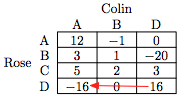
\includegraphics[width=135pt]{img1.jpg}}

But this can't be an equilibrium because if Colin plays A, it is better for Rose to play A, so Rose playing A is a best response to Colin playing A.

\centerline{
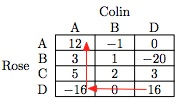
\includegraphics[width=135pt]{img2.jpg}}

Foreseeing this, Colin decides it would be better to play B. But if Colin plays B Rose would play C. If Rose plays C, Colin has no interest to change strategy since choosing A or D he would loose more.

\centerline{
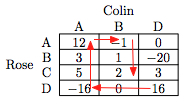
\includegraphics[width=135pt]{img3.jpg}}

So Colin B and Rose C is an equilibrium. Starting from the cell not considered we can repeat the reasoning to check if there are other equilibria. For example starting from the strategy A for Rose and D for Colin we can see that in this case Colin would change strategy to B and now Rose would move to C. Like in the previous case, now Colin has no interest to change. In the end we will come out to the following movement diagram:

\centerline{
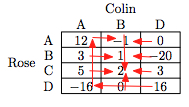
\includegraphics[width=138pt]{img4.jpg}}

The only cell for which we have just in-going edges is the strategy Rose C and Colin B. In this case we have just one Nash Equilibrium, but in general there may be more than one. Zero-Sum-Games have the property that if there are multiple equilibria they are equivalent. This means that at any equilibrium the players  get the same payoff.

The two technique presented are valid also for Non-Zero-Sum games. Let consider the following Non-Zero-Sum game:
\begin{table}
	[H] \centering 
	\begin{game}
		{2}{2}[Anastasia][Andrea] & Scribe & Homework \\
		Scribe & $15,15$ & $13,16$\\
		Homework & $16,13$ & $14,14$\\
	\end{game}
\end{table}

In this game the strategies that players choose correspond to the type of activity they can choose to do, and the payoff is the grade that each one of them gets. The grade doesn't depend just on what a single player choose but also on what the other player choose. If we look for dominated strategies we can see that both for Andrea and Anastasia the Scribe strategy is dominated by the Homework strategy ($15<16$, $13<14$). Hence, we come out to (Homework, Homework) as the unique Nash Equilibrium.\\
We can also build the movement graph. Let's suppose that Andrea and Anastasia are both playing Scribe and let's consider what in this case Andrea and Anastasia would do: 
\begin{itemize}
	\item Anastasia would play Homework, but in this case Andrea would play Homework too and Anastasia would not change strategy 
	\item Andrea would play Homework, but in this case Anastasia would play Homework too and Andrea would not change strategy 
\end{itemize}

\centerline{
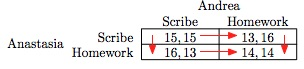
\includegraphics[width=230pt]{img5.jpg}}

We can see from the arrows that they should play both Homework.\\
We can see that the Nash Equilibrium in our case corresponds to the worst set of strategies in terms of social utility. In fact, we have a social utility of 28 against 30 that we could have if they both choose Scribe and 29 that we could have if one of them choose Scribe and the other Homework.\\
The group rationality would tell to prefer one of the outcome between (Scribe, Scribe), (Scribe, Homework) and (Homework, Scribe) but what the individual rationality do is to prefer the outcome (Homework, Homework). So we have a conflict between the interest of the group and the interest of the individuals.\\
In this case we can notice that the outcomes (Scribe, Scribe), (Scribe, Homework) and (Homework, Scribe) are \textbf{Pareto Optimal}, where an outcome $o^*$ is said to be Pareto Optimal if no other outcome would give to all the players a payoff not smaller and a payoff higher to at least one of them.\\
This particular two player Non-Zero-Sum-Game, where the outcome would be better both socially and individually for each player if they would collaborate is well known as \textit{The prisoner's dilemma}. \\
A kind of equilibrium, in which, each time the players play the game, they choose the same strategy is called \textbf{pure strategy equilibrium}. Referring to the last example we can say that (Homework, Homework) is a pure-strategy Nash Equilibrium.\\
Not for all the games there is a fixed strategy that a player should play, for example let us consider the game \textit{Rock-Scissors-Paper}. This game can be represented in normal form by the following matrix:
\begin{table}
	[H] \centering 
	\begin{game}
		{3}{3}[Rose][Colin] & Rock & Scissors & Paper \\
		Rock & $0,0$ & $1,-1$ & $ -1,1$\\
		Scissors& $-1,1$ & $0,0$ & $1,-1 $\\
		Paper & $1,-1$ & $-1,1$ & $0,0$\\
	\end{game}
\end{table}

We can see that there are no dominated strategies, moreover if we build the movement diagram we would have a loop. In this case the unique way for a player to don't loose is to play randomly, that means play Rock, Scissors and Paper according the the probability distribution ($\frac{1}{3}$,$\frac{1}{3}$,$\frac{1}{3}$).\\
In fact, if we play in this way, the other player cannot take advantage of any strategy. If for example Rose would play Rock, Scissors and Paper according the the probability distribution ($\frac{2}{3}$,$\frac{1}{3}$,$0$) Colin would take an advantage by playing Rock, Scissors and Paper according to probability distribution ($0$,$0$,$1$) that means playing Paper all the time. In this case Colin would win $\frac{2}{3}$ of the times and loose $\frac{1}{3}$ of the times.\\
So if Rose and Colin play both Rock, Scissors and Paper according the the probability distribution ($\frac{1}{3}$,$\frac{1}{3}$,$\frac{1}{3}$), no one of them would take advantage by changing his/her probability distribution.\\
When the player plays according to a probability distribution we say that the player is playing according to a \textbf{mixed strategy}.\\
In a mixed strategy equilibrium each player plays a strategy that equalizes the opponent payoff.\\
In the case of Rock-Scissors-Paper when a player plays according to the probability distribution ($\frac{1}{3}$,$\frac{1}{3}$,$\frac{1}{3}$) for the other player it's indifferent to play Rock, Scissors or Paper.\\
\mbox{}\\
Let's consider the following game:
\begin{table}
	[H] \centering 
	\begin{game}
		{2}{2}[Rose][Colin] & A & B \\
		A & $5,0$ & $-1,4$\\
		B& $3,2$ & $2,1$ \\
	\end{game}
\end{table}

In the equilibrium Rose should choose some probability $p$ and $1-p$ such that for Colin playing A or playing B is the same.

If Rose plays A with probability $p$ and B with probability $1-p$ the expected payoff of Colin depends of what he plays.
\begin{itemize}
	\item If he plays A would be: 
	\newline\\
	$\mathbb{E}[U_c|$Rose plays A with probability p and Colin plays A]=$0 \times p + 2 \times (1-p) = 2-2p$ 
	\item If he plays B would be: 
	\newline\\
	$\mathbb{E}[U_c|$Rose plays A with probability p and Colin plays B$]=4 \times p + 1 \times (1-p)= 3p +1$ 
\end{itemize}
\pagebreak Rose should choose $p$ in such a way for Colin it is that same play A or play B that means that solve the equation:\\

\centerline{$2 - 2p = 3p + 1 \Longrightarrow 5p = 1 \Longrightarrow p=\frac{1}{5}$} \mbox{}\\
So Rose should play A with probability $\frac{1}{5}$ and B with probability $\frac{4}{5}$.

In the same way Colin should choose some probability $q$ and $1-q$ such that for Rose playing A or playing B is the same.

If Colin plays A with probability $q$ and B with probability $1-q$ the expected payoff of Rose depends of what she plays.
\begin{itemize}
	\item If she plays A would be: 
	\newline\\
	$\mathbb{E}[U_c|$Colin plays A with probability p and Rose plays A]=$5 \times q - 1 \times (1-q) = 6q-1$ 
	\item If she plays B would be: 
	\newline\\
	$\mathbb{E}[U_c|$Colin plays A with probability p and Rose plays B]=$3 \times q + 2 \times (1-q)= q + 2$ 
\end{itemize}
Colin should choose $q$ in such a way for Rose it is that same play A or play B that means that solve the equation:\\

\centerline{$6q-1 = q + 2 \Longrightarrow 5q = 3 \Longrightarrow q=\frac{3}{5}$} \mbox{}\\
SO Colin should play A with probability $\frac{3}{5}$ and B with probability $\frac{2}{5}$.

If Rose plays A with probability $\frac{1}{5}$ and B with probability $\frac{4}{5}$ and Colin plays A with probability $\frac{3}{5}$ and B with probability $\frac{2}{5}$ then nobody has interest to change probability distribution.\\
This is a \textbf{mixed strategy Nash Equilibrium}.\\
We can calculate the gain of the two players in the equilibrium. To do that we have to calculate the probability distribution of the outcomes: 
\begin{itemize}
	\item $\Pr$(\textit{Rose plays A and Colin plays A})= $\frac{1}{5}*\frac{3}{5}=\frac{3}{25}$ 
	\item $\Pr$(\textit{Rose plays A and Colin plays B})= $\frac{1}{5}*\frac{2}{5}=\frac{2}{25}$ 
	\item $\Pr$(\textit{Rose plays B and Colin plays A})= $\frac{4}{5}*\frac{3}{5}=\frac{12}{25}$ 
	\item $\Pr$(\textit{Rose plays B and Colin plays B})= $\frac{4}{5}*\frac{2}{5}=\frac{8}{25}$ 
\end{itemize}
The gain for Rose would be:\\

\centerline{$u_{Rose}(A,A)*\frac{3}{25} +u_{Rose}(A,B)*\frac{3}{25}+ u_{Rose}(B,A)*\frac{12}{25}+ u_{Rose}(B,B)*\frac{8}{25}$=} \mbox{}\\
\centerline{$=\frac{15}{25}-\frac{2}{25}+\frac{36}{25}+\frac{16}{25}=\mathbf{\frac{13}{5}}$} \mbox{}\\
The gain for Colin would be:\\

\centerline{$u_{Colin}(A,A)*\frac{3}{25} +u_{Colin}(A,B)*\frac{3}{25}+ u_{Colin}(B,A)*\frac{12}{25}+ u_{Colin}(B,B)*\frac{8}{25}$=} \mbox{}\\
\centerline{$=0+\frac{8}{25}+\frac{24}{25}+\frac{8}{25}=\mathbf{\frac{8}{5}}$} \mbox{}\\
\pagebreak

The most important result about the existence of equilibria in games comes from Nash's Theorem.
\begin{theorem}
	[Nash's Theorem, 1950] Every two-person games has at least one equilibrium either in pure strategies or in mixed strategies 
\end{theorem}
This result can be generalized to every game with a finite number of players in which each player can choose from a finite number of strategies.

In a game we could have more than one Nash Equilibrium. Let us consider the \textit{Game of Chicken}. This game involves two drivers, who drive towards each other, and the first one to swerve is considered as a coward (Chicken). In case none of them swerves - they crash into each other.\\
The normal form representation of this game is the following:
\begin{table}
	[H] \centering 
	\begin{game}
		{2}{2}[Driver 1][Driver 2] & swerve & stay \\
		swerve & $0,0$ & $-1,5$\\
		stay & $5,-1$ & $-10,-10$ \\
	\end{game}
\end{table}

Analyzing this game using the movement diagram we would get that there exists two Nash Equilibria. 

\centerline{
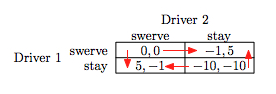
\includegraphics[width=205pt]{img6.png}}

In fact both the outcome (swerve, stay) and (stay, swerve) have just incoming edges. They are clearly not equivalent since Driver 1 would prefer (stay, swerve) and Driver 2 would prefer (swerve, stay), so players have preferences. \\
This is not like for Zero-Sum-Games, for which we have the following 2 properties: 
\begin{enumerate}
	\item if there are multiple equilibria they all yield to the same payoff for each player 
	\item if a player plays a strategy that brings to Nash Equilibrium in pure strategies, always bring to a Nash Equilibrium, whatever the other player decide to play, as long as the other player target a Nash Equilibrium. This property is also called \textit{interchangeability}. 
\end{enumerate}
For Non-Zero-Sum games the two properties don't hold, in the Chicken game we can see the interchangeability property is violated, since if Driver 1 chooses stay and Driver 2 chooses stay they would come out with (stay, stay) that is not a Nash Equilibrium.\\

\section{Auctions} The incentive to study \textbf{Auctions} in our course is to look at another distributed approach to solve the optimization problems. In the lesson 5 we have discussed two different types of users: \textit{price-taking users} - the ones that consider the price as fixed and take it to solve the optimization problem and \textit{price-anticipating users} - rational users, who know how the system is working and exploit it to optimize their problems. The general problem of the network utility maximization was how to let users to reveal their utility. \\
Let us introduce the problem of assigning the good to users in order to maximize the utility. We consider the set of users N, each user $i \in N$ has a value $v_i$ that he assigns to a good. 

\mbox{}\\

Let $x_{i}= 
\begin{cases}
	1 \hfill & \text{ if good is assigned to player \textit{i}} \\
	0 \hfill &\text{ otherwise}\\
\end{cases}
\\
$ \mbox{}\\

\mbox{}\\

\begin{equation*}
\begin{aligned}
& \underset{\mathbf{x}}{\textrm{maximize} }
& & \sum_{i=1}^{N} x_{i}v_{i}\\
& \textrm{subject to } 
	&& \sum_{i=1}^N x_i=1\\
	&&& x_i \in \{0,1\},  \;\; i=1, \dots N \\
\end{aligned}
	\label{e:value_ttil} 
\end{equation*}


\mbox{}\\

The objective functions represents our aim to maximize the sum of the values of the players. The constraints represent the fact that we assign the item to just one player.

Solving this problem we encounter difficulties, such as: 
\begin{itemize}
	\item We do not know the value $v_{i \in N}$ 
	\item We cannot ask users directly, because they have an incentive to lie 
\end{itemize}
As we have already discussed in the course, the way to solve problems with hidden values is to introduce the additional value, that will be represented in our problem by money. \textbf{Auction} is a classical way to distribute goods in exchange for money. Users propose their \textit{bids}, based on the value they give to a good and the good is given to the user with the highest bid. For the purpose of our lecture, we will discuss closed auctions, where the participants do not know the bids of others.\\
\textbf{The game theoretic framework of an auction} consists of: 
\begin{itemize}
	\item A set of N players (bidders) 
	\item Strategies: $b_{i}$ is the bid of the player $i$ 
	\item The value of the good $v_{i}$ for a player $i$, we assume that values $v_i$ are independent and private \textcolor{red}{concepts not defined}
	\item Payment $p_{i}$ if user $i$ gets the good 
\end{itemize}
The utility $U_{i}$ of the user $i$ is defined as: 
\begin{center}
	\mbox{}\\
	$U_{i} = 
	\begin{cases}
		v_i - p_i \hfill & \text{if user $i$ gets the good}\\
		0 \hfill & \text{otherwise}\\
	\end{cases}
	$\\
	\mbox{}\\
\end{center}
As compared to the classical game theory model, in our case it is better to model the strategy space as continuous, because the distribution of possible bids is unknown. 
\subsection{Types of auctions}

\subsubsection{\nth{2}-price ascending bids auctions } The idea of the second price auction is that players bid independently and privately of each other, and after the collection of results, the player with the highest bid will get the good, but will pay the \nth{2} highest bid. This type of auctions is called \textbf{ascending bids auctions} or \textbf{English auctions}. \textcolor{red}{Not correct, ascending bids auctions are different from 2nd price, but they are equivalent for our purposes.} \\
\textcolor{red}{There was some misunderstanding about the following example, it has been significantly rewritten, pay attention.}
Let us see the following example of one-item auction. Let us consider player $i$. We want to show that, independently from the other players' bids, $b_i=v_i$ is a dominant strategies. Firstly, we will consider the case, where player $i$ happens to be the highest bidder. According to the rules of \nth{2}-price auctions, the initial utility of the player $i$ was $U_i=v_i-b_k$ that is equal to the difference between the value of a good for the user $i$ and the amount of money he will pay for the good, which is the second highest bid $b_k$. In the case 1, presented on the Figure~\ref{fig:bids1}, after changing his bid to a higher one, the player $i$ will still win the good and his utility $U_i=v_i-b_k$ will not change not depending on the increment in his bid. 
\begin{figure}
	[!hbt] 
	\begin{center}
		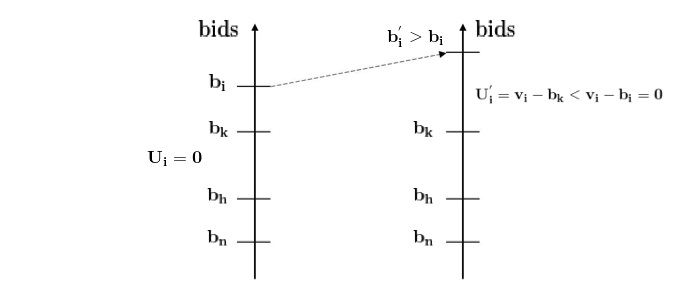
\includegraphics[height=5cm]{img7.jpg} \caption{An example of one-item auction. Case 1: The highest bidder decides to raise the bid.} \label{fig:bids1} 
	\end{center}
\end{figure}

In the case~\ref{fig:bids2}, we consider a situation, where the player $i$ decides to lower his bid $b_i$. Since all bids are private, he doesn't know whether this change will affect the outcome of the auction. Let us consider an example, where $b'_i<b_i$. The highest bidder will loose the good, and his utility will be equal to zero. We conclude that bidding less than the value of the good $v_i$ is not convenient in this case.
\begin{figure}
	[!hbt] 
	\begin{center}
		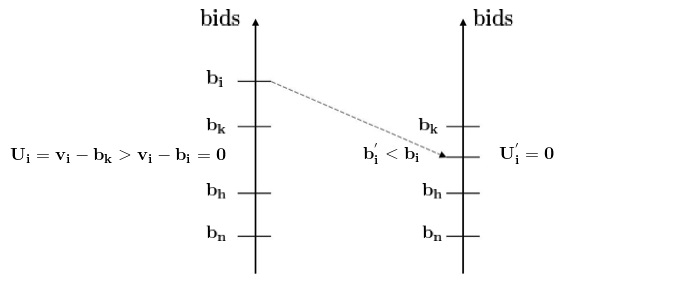
\includegraphics[height=5cm]{img8.jpg} \caption{An example of one-item auction. Case 2: The highest bidder decides to lower the bid.} \label{fig:bids2} 
	\end{center}
\end{figure}

Now, let us know consider the case when player $i$ is not the highest bidder, but, for example, he is the second highest bidder. On the Figure~\ref{fig:bids3}, we see the case when he decides to raise his bid in a way that it will be higher than all other bids. Before raising the bid, the utility of a player $i$ was equal to zero, because he was not able to get the good. After raising his bid $b'_i>b_i>b_k$, the utility will become negative, because $U'_i=v_i-b_k<v_i-b_i=0$. We conclude that bidding more than the value of the good in this case is not convenient.
\begin{figure}
	[!hbt] 
	\begin{center}
		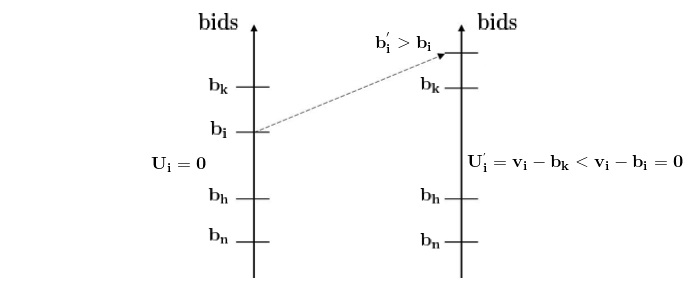
\includegraphics[height=5cm]{img9.jpg} \caption{An example of one-item auction. Case 3: The second highest bidder decides to raise the bid.} \label{fig:bids3} 
	\end{center}
\end{figure}

Finally, let us take a look at the case~\ref{fig:bids4} where  bidder $i$ lowers his bid in a way that $b'_i<b_i=v_i$. The utility $U'_i=U_i=0$ doesn't change, so we see that in this case it is also not convenient to bid less than the value of the good.

To conclude, we saw that in any case in \nth{2}-price auctions, bidding differently from the value of the good is not a good strategy since it doesn't allow the players to increase their utility. For the players that bid more than they value the good there is a risk to get the negative utility in case they will get the good by paying more than their value. 
\begin{figure}
	[!hbt] 
	\begin{center}
		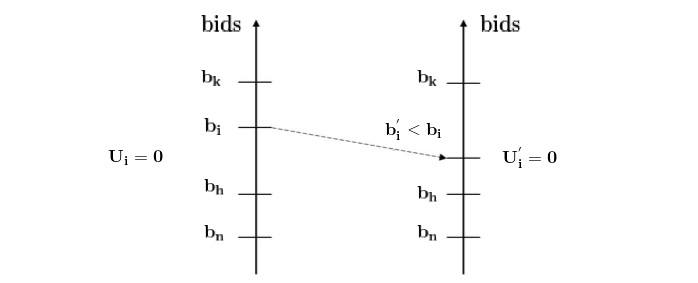
\includegraphics[height=5cm]{img10.jpg} \caption{An example of one-item auction. Case 4: The second highest bidder decides to lower the bid.} \label{fig:bids4} 
	\end{center}
\end{figure}

The \textbf{dominant} strategy in the \nth{2}-price auction is to be truthful, i.e. to set $b_i = v_i$, because as we have seen, whatever other strategy does not lead to an improvement of the utility $U_i$. Moreover, it is socially optimal, due to the fact that the player that values the good the most gets it.\\
Now let us consider the gain of the seller. To calculate the expected utilities, let us consider that $u_{i \in N}$ is an independent random variable, such that $U_i \in \{0,1\}$ and assume moreover that bidders have been renamed so that $U_1 \ge U_2 \ge \dots U_N$. The seller gains the second highest bid according to the rules of the \nth{2}-price auctions. To calculate the expected gain of the seller, we consider the expected utility of a player $i$ to be: 
\begin{equation}
	\mathbb{E}[U_i] = \frac{(N + 1 - i)}{(N + 1)}, 
\end{equation}
where N is the total number of players. Given N bids as a point in an interval we have N+1 intervals, and on average the highest bid would be in the interval N over N+1, the second biggest bid in the interval N-1 over N+1 and so on. Since the seller gets the second largest bid, its revenue could be expressed as: 
\begin{equation}
	\mathbb{E}[R_s] = \frac{N-1}{N+1} 
\end{equation}
This is supported by the fact that, the more players there are in the auction, the more they will compete for the good, and the seller revenue $R_s$ will converge to 1, with the increasing number of players.

\subsubsection{\nth{1}-price or descending bids auctions } The idea of the first price auction is that players bid independently and privately of each other, and after the collection of results, the player with the highest bid will get the good, and will pay his own bid. This type of auctions is called \textbf{descending bids auctions} or \textbf{Dutch auctions}. \textcolor{red}{As above: this is not correct, descending bids are technically different auctions but they are equivalent for our purposes.}\\
\sout{The hypothesis that we can make about the \nth{1}-price auctions is that, unlike in the case of \nth{2}-price auctions being truthful is not a dominant strategy anymore.} \textcolor{red}{This statement was wrong, it is not a hypothesis, it is a fact. There was also some misunderstanding later about the calculation of the NE, the text has been changed} In \nth{1}-price auctions being truthful is not a dominant strategy anymore. In fact, assume that every player is being truthful, the highest bidder would then find convenient to lower his bid to pay less. 

Under the following hypotheses
\begin{itemize}
	\item Each player knows the total number of players N 
	\item The utilities of all players are independent and identically distributed random variables, such that $u_{i \in N} \in \{0,1\}$
\end{itemize}
it is possible to prove that there is a Nash equilibrium, in case all players bid as follows: 
\begin{equation}
	b_i = \frac{N-1}{N} v_i 
\end{equation}
The expected seller revenue in the case of the \nth{1}-price auction depends on the top highest bid (differently from the \nth{2}-price auctions). Since the players tend to bid less than they value the good, depending on the total number of players, the expected revenue of the seller is: 
\begin{equation}
	\mathbb{E}[R_s] = \frac{N-1}{N}\mathbb{E}[v_{max}] = \frac{N-1}{N} * \frac{N}{N+1} = \frac{N-1}{N+1} 
\end{equation}

As we can see, expected seller revenue is the same as for the \nth{2}-price auction. This is called a \textbf{general revenue equivalence principle. }\\
We observe that, in the case of the \nth{1}-price auction, the dominant strategy is not to be truthful, but to bid less than the value of a good and this strategy leads to the Nash equilibrium. 

\section{Matching markets} Suppose now to have multiple goods and in particular that there are $N$ buyers and $N$ goods.\\
Each buyer assign a value to each good.\\
We define $v_{ij}$ as the value that buyer $j$ gives to good $i$. Clearly these values can be different.\\
We would like to assign goods to buyers in such a way to maximize the social utility.\\
This problem can be modeled as a linear program.

\mbox{}\\

Let $x_{ij}= 
\begin{cases}
	1 \hfill & \text{ if good \textit{i} is assigned to buyer \textit{j}} \\
	0 \hfill &\text{ otherwise}\\
\end{cases}
\\
$ \mbox{}\\
The problem can be formulated in the following way:
\begin{equation*}
%	\begin{array}{ll@{}
%		ll} \text{maximize} & \displaystyle\sum\limits_{i=1}^{N}\sum\limits_{j=1}^{N} x_{ij}&v_{ij} &\\
%		\text{subject to}\\
%		& \displaystyle\sum\limits_{j=1}^{N} &x_{ij} = 1, &i=1 ,..., N \\
%		& \displaystyle\sum\limits_{i=1}^{N} &x_{ij} = 1, &j=1 ,..., N\\
%		& &x_{ij} \in \{0,1\}, &i=1,...,N \text{ } j=1,...,N 
%	\end{array}
%
\begin{aligned}
& \underset{X}{\textrm{maximize} }
& & \sum_{i=1}^{N}\sum_{j=1}^{N} x_{ij}v_{ij}\\
& \textrm{subject to } 
	&& \sum_{j=1}^N x_{ij}=1, \;\; i=1, \dots N \\
	&&& \sum_{i=1}^N x_{ij}=1, \;\; j=1, \dots N \\	
	&&& x_{ij} \in \{0,1\},  \;\; i,j=1, \dots N \\
\end{aligned}
\end{equation*}
\mbox{}\\
The objective function expresses our purpose to maximize the sum of the values that each buyer would have in the assignment.\\
The first set of constraint expresses the fact that each good is assigned to just one buyer.\\
The second set of constraint express the fact that to each buyer is assigned just one good.

As in the previous case we can't ask buyers about the value that they give to each good because they could lie since there is no incentive for them to say the truth. So like in the auction case we need to introduce money in the form of prices.

We can assign a price $p_i$ to each good $i$, and ask the the buyers which good they prefer.\\
Each buyer $j$ by computing $v_{ij}-p_i$ can calculate the utility that he would get if he acquired the good $i$ and will answer with the good (or goods in case they are more than one) that allow him to get the maximum utility. Based on the answers we can build a \textit{preference graph}.

Let us consider the following example:

\centerline{
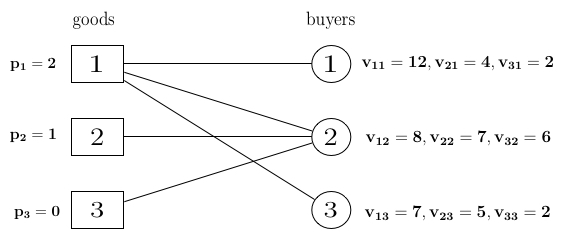
\includegraphics[width=300pt]{img12.jpg}}

In this case buyer 1 would prefer good 1 since his payoffs based on the prices are $(10,3,2)$ and good 1 give him the maximum payoff. For buyer 2 it's equivalent to get good 1, 2 or 3 since his payoff are $(6,6,6)$. Buyer 3 would prefer good 1 since it's the one that gives him the higher payoff, in fact his payoff are $(5,4,2)$.\\
Given these preferences we draw an arrow between each buyer and his preferred good (or goods). A perfect matching in the graph would be an assignment of goods to buyers. Unfortunately, the graph of our example does not have a perfect matching. What we can try to do is to change the prices. For example, let's increase the price of $p_1$ from 2 to 3. The new preference graph, due to this change, would be different:

\centerline{
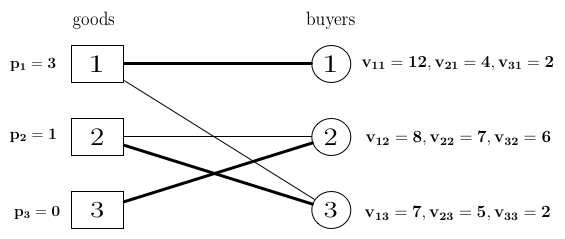
\includegraphics[width=300pt]{img13.jpg}}

In fact now buyer 2 would not prefer anymore good 1 since his payoffs now are $(5,6,6)$ and buyer 3 would prefer not just good 1 but also good 2 since his payoffs now are $(4,4,2)$. Even if the price for good 1 has changed buyer 1 continues to prefer just good 1.\\
In this graph we can find a perfect matching that in the case of the graph corresponds to the assignment: 
\begin{itemize}
	\item good 1 to buyer 1 
	\item good 2 to buyer 3 
	\item good 3 to buyer 2 
\end{itemize}

The total social utility for this assignment would be:\\

\centerline{$v_{11}+v_{23} +v_{32}=12+5+6=23$} \mbox{}\\
and it is optimal is the sense that we can't find any other assignment that would give has a higher social utility.

The prices so determined are called \textbf{Market Clearing Prices}. Market Clearing Prices are those prices that allow to assign all the goods in the market (that means find a perfect matching) and they achieve the maximum total valuation of any assignment of sellers to buyers. Two important properties of the Market Clearing Prices are that they always exist and that they maximize the global payoff for both sellers and buyers but, to calculate Market Clearing Prices, we need to know the valuations of the buyers. 
\section{Approaches for the advertisement pricing} In this last section we will try to put together the \textit{matching market}, where we know that Market Clearing Prices exist, and \textit{auctions}, where we want to define a mechanism that brings the bidders to reveal the real value that they assign to each good.\\
The problem for an advertising company like \textit{Google} is to find a matching bewteen advertisements (ads) position and companies. We can assign to each position a value $r_i$ defined as the click rate for an ad in position $i$. This rate is known a priori. Each company has a value $v_i$ defined as the value that company $i$ gives to a click. Knowing this information we would be able to calculate the value of a given position for each company. In fact, the value of $r_i$ click for company $i$ is given by $v_i*r_i$.\\
We would have the following problem:

\centerline{
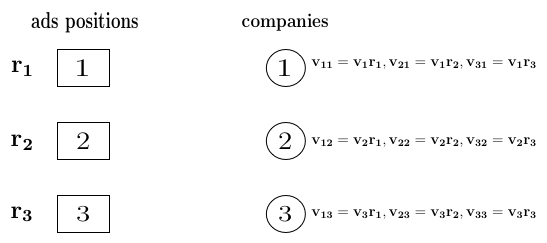
\includegraphics[width=300pt]{img14.jpg}}

As we can see the problem would become the same as the Matching Market that is to find Market Clearing Prices. To do this we need to know the value $v_i$ for each company. What we can do it to set up an auction where companies bid the value for a click $b_i$ and we assign the $N$ ads positions $r_1,...,r_N$ to the companies considering their $b_i$ in non increasing order: the best position is assigned to the company that has bid the most, the second best position is assigned to the company that has bid the second value and so on.\\
We saw in section 3 that \nth{2} price auction is a truthful mechanism in case of single item auction.\\
We would like to generalize this mechanism for multiple items auction.\\
The first idea could be to use the natural extension of the \nth{2} price auction in which the highest bidder gets the first position and pays the price bid by the second-highest bidder, the second-highest gets the second position and pays the price bid by the third-highest bidder, and so on. This mechanism is called \textbf{Generalized second-price auction} or \textbf{GSP}. Unfortunately GSP is not a truthful mechanism.\\
The correct way to generalize the \nth{2} price auction that provides us a truthful mechanism is the \textbf{VCG} (Vickrey-Clarke-Groves). In a VCG auction every buyers should pay a price equal to the social value loss for the others buyers. This means that a buyer should pay the difference between what the other players would have got if he were not be there and what they  get if he is there.\\
Suppose to have an auction for a single item and that the bids are such that $b_1>b_2>...>b_N$; so buyer 1 would get the item. Let us consider the social utility for the buyers $2,3,...,N$: 
\begin{itemize}
	\item if buyer 1 is not present it would be $v_2$ ($b_2=v_2$ being VCG a truthful mechanism). In this case buyer 2 would get the item since by hypothesis $b_2$ is the second highest bid, the other buyers ($3,...,N$) would have an utility equal to $0$ because of the the fact that they don't get the item. 
	\item if buyer 1 is present it would be 0, since buyer 1 get the item and for all the other, since no one of them get the item, the utility would be $0$ 
\end{itemize}
So for single item auction the winner should play $v_2-0=v_2$. VCG in the case of single item auction become the \nth{2} price auction. Moreover, $v_2$ is not just the second price but it's also the damage done to the society.\\
In case of multiple items auction, let $V_{B}^{S}$ be the maximum total valuation over all the possible perfect matchings between the set of sellers S and the set of buyers B. If buyer j gets good i, he should pay the difference between the total valuation that the other people get if j would not be there dividing by them the set of goods ($V_{B-j}^{S}$) and the total valuation that the other people get if j would be there ($V_{B-j}^{S-i}$) dividing by them the set of goods except good i. Under this price mechanism, truth-telling is a dominant strategy.

Let's make an example. There are 3 ads position with a click rate of $10$ for \nth{1} position ($r_1=10$),$5$ for \nth{2} position ($r_2=5$) and $2$ for \nth{3} position ($r_3=2$). Moreover we have 3 companies for which the values of a click is 3 for company 1 ($v_1=3$), 2 for company 2 ($v_2=2$) and 1 for company 3 ($v_3=1$).\\
These informations are enough to calculate the value that each company gives to each position.

\centerline{
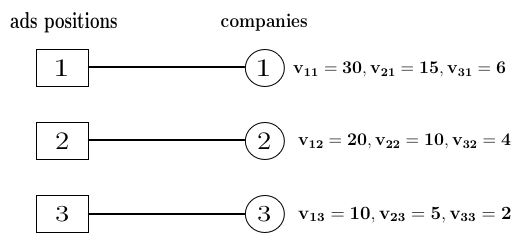
\includegraphics[width=300pt]{img15.jpg}}

Moreover we can see that the maximum weight perfect matching is the one that assign position 1 to company 1, position 2 to company 2 and position 3 to company 3. This assignment gives us a total valuation of $42$ (so $V_{B}^{S}=42$). In fact company 1 gets 30, company 2 gets 10 and company 3 gets 2. 

Now let's calculate how much each company should play according to VCG mechanism. 
\paragraph{Company 1} \mbox{}\\
In our optimal allocation the total valuation that companies 2 and 3 get if company 1 participate is 12. But if company 1 did not participate we would have the following allocation for companies 2 and 3

\centerline{
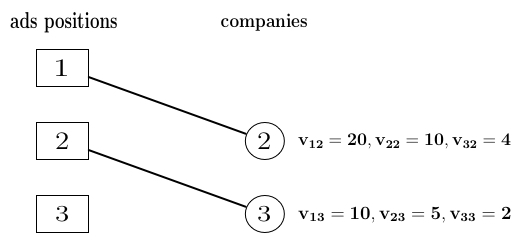
\includegraphics[width=300pt]{case1.jpg}}

So if company 1 did not participate the total valuation that companies 2 and 3 get would be 25. So company 1 should pay $V_{B-1}^{S}-V_{B-1}^{S-1}=25-12=13$

\paragraph{Company 2} \mbox{}\\
In our optimal allocation the total valuation that companies 1 and 3 get if company 2 participate is 32. But if company 2 did not participate we would have the following allocation for companies 1 and 3

\centerline{
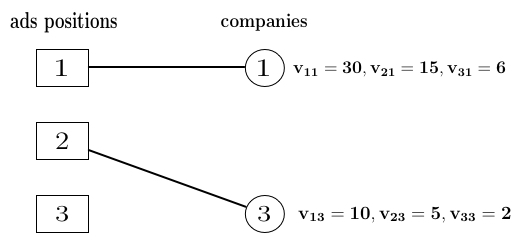
\includegraphics[width=300pt]{case2.jpg}}

So if company 2 did not participate the total valuation that companies 1 and 3 get would be 35. So company 1 should pay $V_{B-2}^{S}-V_{B-2}^{S-2}=35-32=3$

\paragraph{Company 3} \mbox{}\\
In our optimal allocation the total valuation that companies 1 and 2 get if company 3 participate is 40. But if company 3 did not participate we would have the same allocation for companies 1 and 2

\centerline{
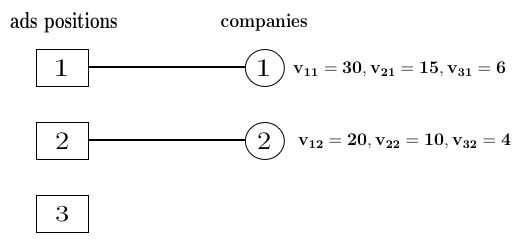
\includegraphics[width=300pt]{case3.jpg}}

So if company 3 did not participate the total valuation that companies 1 and 2 get would be 40. So company 1 should pay $V_{B-3}^{S}-V_{B-3}^{S-3}=40-40=0$

\section{Conclusion} In this lesson we have studied the basics of the \textit{Game theory}. We introduced tho types of two player games: \textit{Zero-Sum-Games}, where the payoff for users is strictly opposite and \textit{Non-Zero-Sum-Games}, where payoff is not necessarily opposite. We introduced the notion of \textit{Nash Equilibrium} as a set of players' strategies, such that there is no interest for any players to change their strategies unilaterally. We saw that there could be multiple equilibria, and, in case of the Zero-Sum-Games, those equilibria are equivalent, as opposed to the Non-Zero-Sum-Games, where different players could prefer  different equilibria. In this case it is not clear which strategy each player should target, if they target different strategies they could achieve a worst payoff. The Nash equilibrium can be in \textit{pure strategies} when, each time the players play the game, they choose the same strategy and in \textit{mixed strategies} when the players choose a strategy according to a probability distribution.\\
Then, we applied the notions of the game theory on the particular model - \textit{auctions}. Auctions are a convenient way to study distributed optimization problems, where the goal is to maximize the social utility by introducing money. We introduced two types of auctions: \nth{1}-price and \nth{2}-price. In case of the \nth{2}-price auction, we saw that the dominant strategy of an each player is to be truthful, i.e. to bid exactly his value of the good. As an oppose, for the \nth{1}-price auctions, the best strategy is to bid less than the value of the good. \\
We looked at \textit{Matching Markets}, i.e.~the problem to match a given set of goods to an equally large set of buyers. By knowing the valuations of the buyers we can find \textit{Market Clearing Prices} that will allow us to assign all the goods in the market and to achieve the maximum total valuation for both sellers and buyers.\\
We concluded by trying to put together matching market and auctions with the goal to find a assignment of advertisements position to companies. We saw that, if we want to assign the advertisements positions with the goal of maximizing the sum of valuations we can use Market Clearing prices. Since we can't ask companies directly, to find those values we can set up an auction and make companies pay truthfully, according to the \textit{VCG} mechanism. According to VCG, each company should pay a price equal to the social value loss for the others companies. By using this mechanism companies dominant strategies would be to reveal the real value of a click. 

%%%%  Bibliography goes here
\begin{thebibliography}
	{alpha}
	
	\bibitem{Netw} David Easley and Jon Kleinberg, 
	\newblock Networks, Crowds, and Markets: Reasoning about a Highly Connected World. 
	\newblock {\em Cambridge Press}, 2010.
	
	\bibitem{GTDC} J. R. Marden and J.S. Shamma, 
	\newblock Game Theory and Distributed Control, Handbook of Game Theory Vol. 4, edited by Peyton Young and Shmuel Zamir. 
	\newblock {\em Elsevier Science}, 2013.
	
	\bibitem{Nagle} John Nagle, 
	\newblock RFC 970, On Packet Switches With Infinite Storage. 
	\newblock {\em FACC Palo Alto}, 1985.
\end{thebibliography}

\end{document}
